\documentclass[12pt]{article}
\usepackage{amsmath}
\usepackage{amssymb}
\usepackage{hyperref}
\usepackage{graphicx}
\usepackage[utf8]{inputenc}
\usepackage[english]{babel}
\newcommand{\R}{\mathbb{R}}

\title{Algorithmic Operation Research \\ Homework 2}
\date{25-10-2019}
\author{Theodora Panagea - 1115201400135 \\ Anna-Aikaterini Kavvada - 1115201500050}

\begin{document}
	\maketitle{}
  	\pagenumbering{arabic}
  	
%-------------------Exercise 1--------------------------

\subsection*{Exercise 1}
\textit{Find a differentiable function $f: \R \rightarrow \R$ such that $f$ does not have an extremum at its critical point. }\\
\textbf{Solution:} \par
The critical point is defined as follows: \\
For a differentiable function $f :\R \rightarrow \R$,  $\exists  x_0 \in \R$  so that $f'(x_0) = 0$ or $\nexists f'(x_0).$ \\
If we consider the function: \\
$$f(x) = 
  \begin{cases} 
      x & x < 0 \\
      5x &  x \geqslant 0 
   \end{cases}
$$ \\
we notice that the $f$ is differential, but for $x_0 = 0$, $f'$ doesn't exist, so $x_0$ is a critical point. However, $f(x_0)$ is not an extremum. 
\newpage

%-------------------Exercise 2--------------------------

\subsection*{Exercise 2}
\textit{Given a positive integer $S$, which decompositions  \\
$$a_1+\cdots+a_n = S$$ \\
with the $a_i$ positive integers have the largest product $a_1 \cdots a_n$ ? }\\
\textbf{Solution:} \par
Assume that any $a_k$ of the $a_i$ is greater than 4. We could then subsitute this number by $\frac{a_k}{2} + \frac{a_k}{2},$ which has a product greater than $a_k$, since \\
 $$(\frac{a_k}{2})^2 \geqslant a_k \Leftrightarrow a_k \geqslant 4.$$ \\
 If $a_k$ is odd, we do the same method but with 2 numbers with difference 1. \\
 From this, we can conclude that there can be no numbers greater than 3 in our sum. Also, there can be no 1s for obvious reasons.  \par
 Hence, we have a selection of $x$ 3s and $y$ 2s, where $3x+2y \leqslant S.$ Formally, we have to look at the cases $3x + 2y = S$ and $3x+2y = S-1,$ since if the sum was less or equal than $S-2$, we could simply add 2. \\
 In accordance to the aforementioned, we can write our product as: \\
 $$3^x2^{\frac{S-3x}{2}}$$\par
 For example, if $ S = 100,$ then, if we look at the above function and its maximum properties, the only possible values for a maximum product are $x = 32$ and  $x = 33$. Comparison leads to the maximum being at $x = 32$ and $y = 2$. \par
 Finally, we cannot have more than 3 2s, because we could substitute them with 2 3s, since $3^2 \geqslant 2^3$.
\newpage

%-------------------Exercise 3--------------------------

\subsection*{Exercise 3}
\textit{Find the optimal solution to the Diet Problem when the cost function is}\\
$$Cost(x_1, x_2) = x_1 + x_2.$$  
\textbf{Solution:} \par
Consider we have 2 products, Product1 and Product2, which contain 2 elements, Element1 and Element2. We buy $x_1$ of Product1 and $x_2$ of Product2. The Product1 provides 30 of Element1 and 15 of Element2. The Product2 provides 5 of Element1 and 10 of Element2. The constraints we have, are the following: \\
$$30x_1+5x_2 \geqslant 60$$ 
$$15x_1+10x_2 \geqslant 70$$ \\
Needless to say, both quantities need to be non-negative integers. \par
We notice that since the price for both products is 1, it's better to buy the Product1, since it contains more quantity of the elements than Product2, for the same price. Thus, we can compute that we will need 5 items of Product1, which gives us 150 Element1 and 75 Element2. Both our constraints are met. \par 
A different approach would be to draw a picture of the constraints and the cost function, as it is shown on Figure 1.

\begin{center}
	\begin{figure} 
        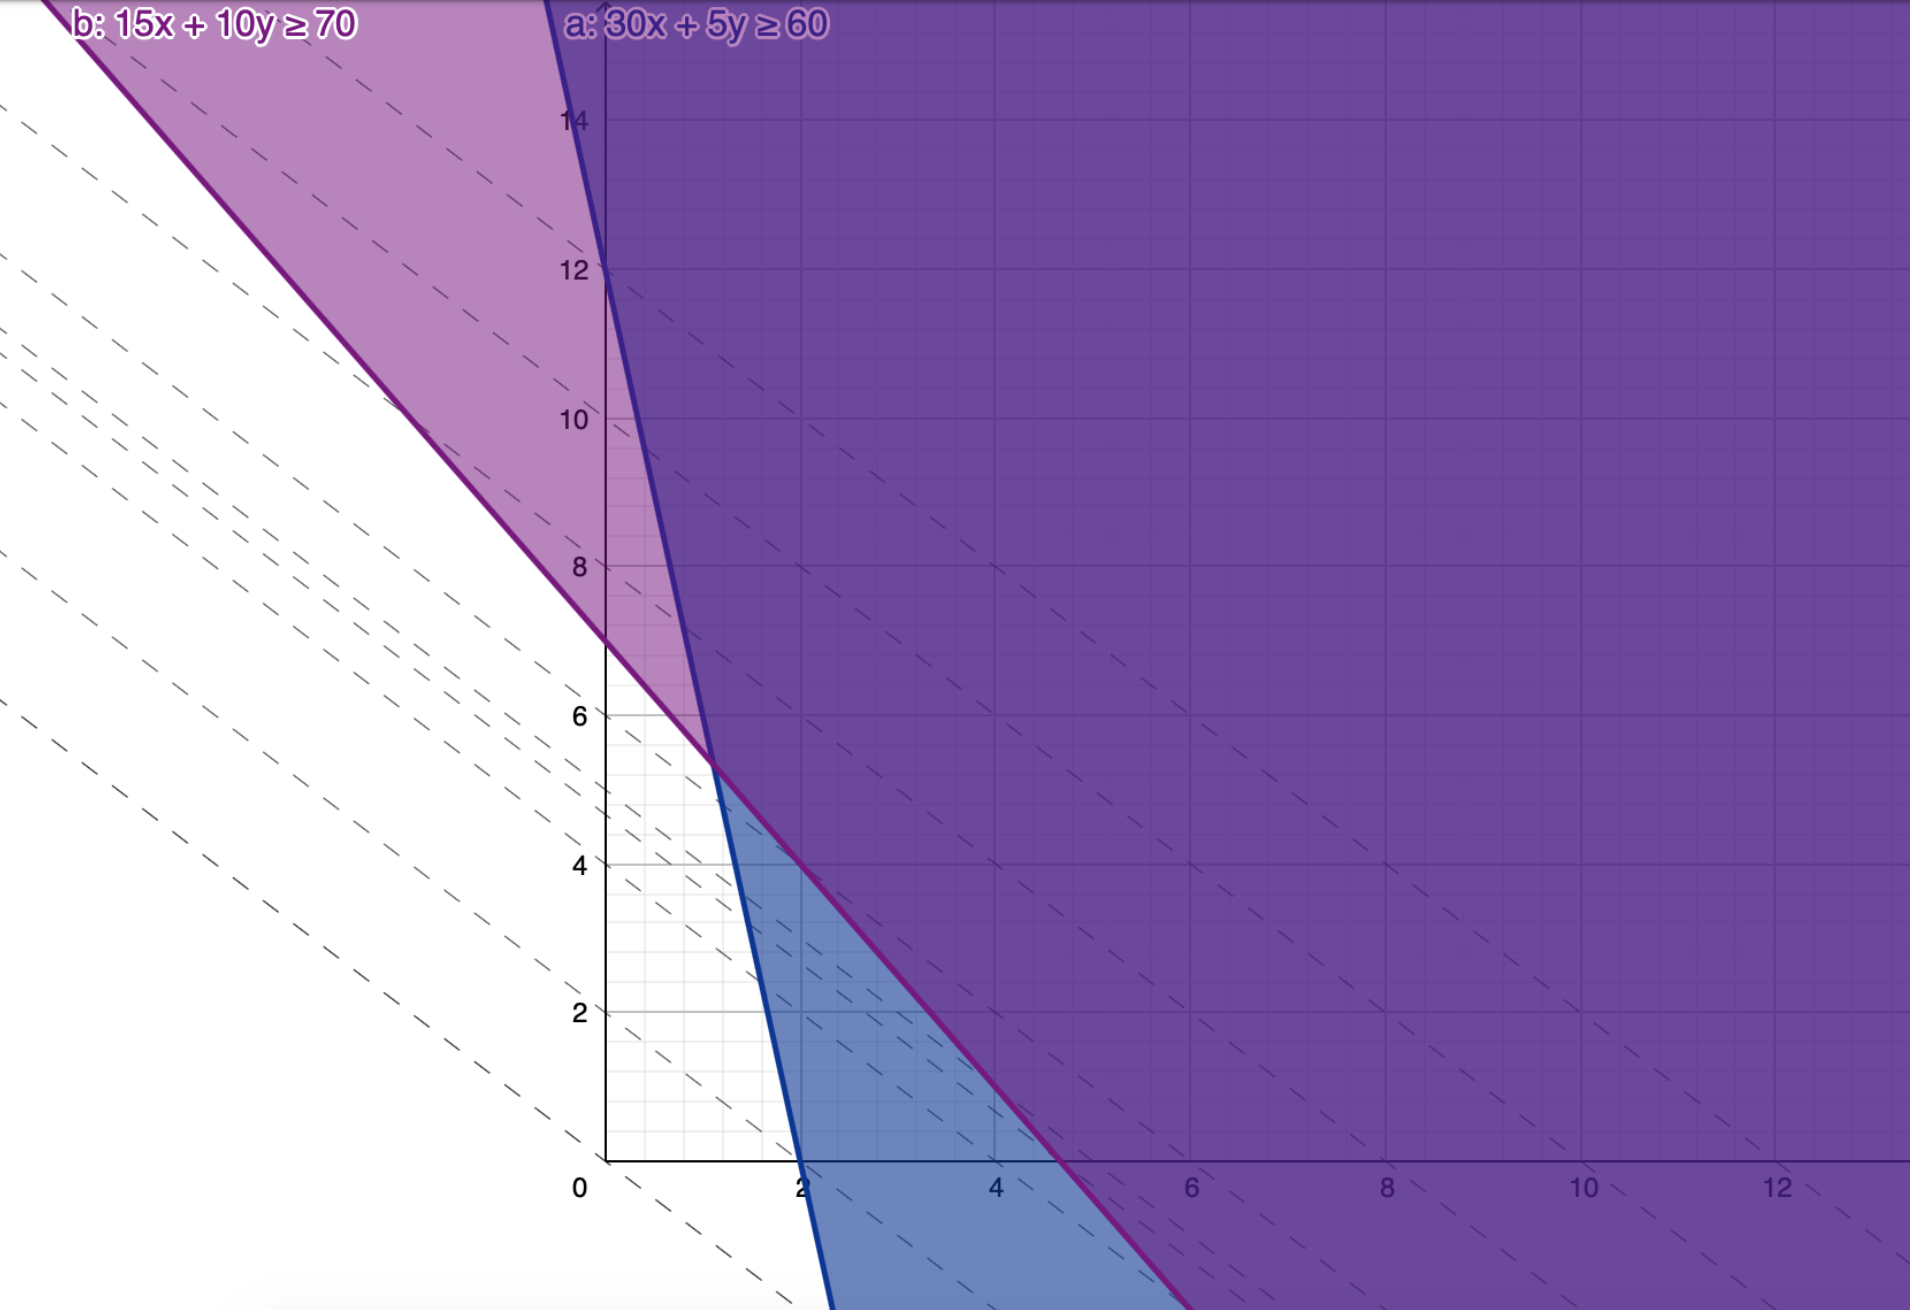
\includegraphics[totalheight=8cm]{figure.png}
		\caption{Graphic Representation}	
	\end{figure}        
\end{center} 
\newpage

We can also use the tool "Solver" from Excel. The above example is implemented in the following link: 
\url{https://docs.google.com/spreadsheets/d/1pejhOMkti4tc715EH77R8OGJunuIkjl3Mu1uETAt664/edit?usp=sharing} . If the Solver doesn't show up, please click on the "Add-ons" on the navigation menu, and select "Document Add-ons".

\newpage

%-------------------Exercise 4--------------------------

\subsection*{Exercise 4}
\textit{Let $A, B \in \R^{nxn}$. Show that the traditional way of computing their product $AB$ requires a total of $(2n-1)n^2$ arithmetic operations.}\\
\textbf{Solution:} \par
It is known that the formula for computing the product of $2$ matrices $C = AB$, with $A,B \in \R^{nxn},$ is: \\
$$c_{ij}= \sum_{s=1}^{n} a_{is}b_{sj}$$
Thus, we need: \par
$\bullet$ $n$ comparisons for $i$ \par
$\bullet$ $n^2$ comparisons for $j$ \par
$\bullet$ $n^3$ comparisons for $s$ \par
$\bullet$ $n^3$ computations to find the sum. \\ \\
Therefore, 
$$2n^3 + n^2 + n =$$
$$= 2n^3 + 2n^2 - n^2 + n =$$
$$=  n^2(2n-1) + n(2n+1) $$
It is obvious that $$n^2(2n-1) \geqslant n(2n+1).$$
So, the complexity of this operation, is $n^2(2n-1).$


\newpage

%-------------------Exercise 5--------------------------

\subsection*{Exercise 5}
\textit{Consider the problem of solving a system of $n$ linear equations in  $n$ unknowns. Show that the Gaussian elimination method requires $\mathcal{O}(n^3)$ arithmetic operations in order to either compute a solution or to decide that no solution exist.}\\
\textbf{Solution:} \par

So basically, we hace an $nxn$ matrix and want to apply the Gaussian elimination method, to prove that it requires $\mathcal{O}(n^3)$ arithmetic operations, in order to either compute a solution or decide that there is none. \par 
From linear algebra, a $nxn$ system of linear equations has a unique non-trivial solution if and only if its determinant is non-zero. If the determinant, is zero, then the system has either no nontrivial solutions or an infinite number of solutions. \par 
Furthermore, if Gaussian elimination is applied to a square matrix $A$, it produces a row echelon matrix B, let d be the product of the scalars by which the determinant is multiplied. Then the determinant of A is the quotient by d of the product of the elements of the B's diagonal: 
$$det(A) = \frac{\prod diag(B)}{d}$$
The variable d is computed by the following rules: \\
\textbf{1.}Swapping two rows multiplies the determinant by $-1$. \\
\textbf{2.}Multiplying a row by a nonzero scalar, multiplies the determinant by the same scalar. \\ 
\textbf{3.}Adding to one row a scalar multiple of another, does not change the determinant. \\ \\
Computationally, for a $nxn$ matrix, this method needs only $\mathcal{O}(n^3)$ operations. 
\newpage

%-------------------Exercise 6--------------------------

\subsection*{Exercise 6}
\textit{Suppose that we are given a set of vectors in $\R^n$ that form a basis and let $y$ be an $n$ arbitrary vector in $\R^n$. We wish to express $y$ as a linear combination of the basis vectors. How can this by accomplished?}\\
\textbf{Solution:} \par
Let's define the vectors: \\
\begin{center}
$\bullet$ $\overrightarrow{e_1} := (1,0,\ldots,0) \in \R^n$ \\
$\bullet$ $\overrightarrow{e_2} := (0,1,\ldots,0) \in \R^n$ 
$$\vdots$$ 
$\bullet$ $\overrightarrow{e_n} := (0,0,\ldots,1) \in \R^n$
\end{center}
The $\lbrace \overrightarrow{e_1}, \overrightarrow{e_2}, \ldots, \overrightarrow{e_n}\rbrace$ are linearly independent and
$$\forall \overrightarrow{y} = (y_1, y_2, \ldots, y_n) \in \R^n$$
we have
$$\overrightarrow{y} = y_1 \overrightarrow{e_1} + y_2 \overrightarrow{e_2} + \cdots + y_n \overrightarrow{e_n}.$$
Thus, $\lbrace \overrightarrow{e_1}, \overrightarrow{e_2}, \ldots, \overrightarrow{e_n}\rbrace$ is an $\R^n$ basis. \\
So we can use this basis vectors, to express an arbitrary vector $\overrightarrow{y}$ in $\R^n$ as linear combinations of the basis. 
\newpage

%-------------------Exercise 7--------------------------

\subsection*{Exercise 7}
\textit{Study the paper with title: "Do dogs know Calculus?" found in the Readings folder.}\\
\textbf{Solution:} \par
\textbf{Solution:} \par
{Below follows a small presentation of the paper "Do dogs know claculus", written by Timothy J.Pennings.\\
The problem this paper refers to can be categorized as an \textit{optimal path} problem. For a path to be optimal, it may be that we minimize the travel time between the two points (start point (A), end point (B)), while taking into consideration that the available paths must transverse two different mediums, involving different rates in speed.\par 
In this paper, we apply the above on Elvis' case (Elvis' being the author's corgi). Thus, we have Elvis who seems to be determined every time to fetch his ball as quickly as possible, without caring about the energy expenses he might suffer. This, leads us to the assumption that Elvis, unconciously tries to "calculate" the optimal path to minimiae the balls retreival time.\par 
\begin{center}
\textbf{The situation}
\end{center}
We are standing on the water's edge (point A) of Lake Michigan to play fetch the ball with Elvis. After the tennis ball we use, ends up at point B, as shown in the figure below.
\begin{figure}[h!]
  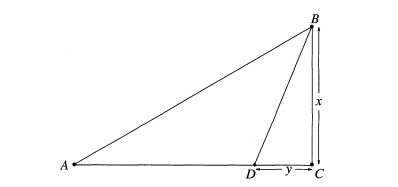
\includegraphics[width=\linewidth]{pathsToTheBall.png}
  \caption{Paths to the ball.}
  \label{fig:path1}
\end{figure}
\begin{center}
\textbf{What is Elvis' strategy?}\\  
\end{center}
$\textbf{1.}$ Minimize retrieval time by minimizing the distance\\
$\textbf{2.}$ Minimize swimming distance since $u_{run} > u_{swim}$ \\
$\textbf{3.}$ Running a portion of the way and swimming the rest \\ $\newline$
\textbf{Note:}Option 3, usually turns out to minimize the time (depends on the relative $u_{run}$ and $u_{swim}$)
\begin{center}
\textbf{Solve the problem $\rightarrow$ General Case}\\
\end{center}
$\bullet r = u_{run}$: running speed\\
$\bullet s = u_{swim}$: swimming speed\\
$\bullet$ units used: meters and seconds\\
$\bullet T(y)$:time to get to the ball, given that Elvis jumps into the water at D\\
$\bullet z = (AC)\newline$\\ 
We have\\ $$\newline T(y) = \frac{z-y}{r} + \frac{\sqrt{x^2 + y^2}}{s} \quad (1)$$\\
For $T'(y)= 0$, we calculate the minimum value for the equation. Solving $T'(y) = 0$ for $y$, we get 
$$y  = \frac{x}{\sqrt{\frac{r}{s}+1}\sqrt{\frac{r}{s}-1}} \quad (2)\newline$$\\ 
\textbf{Note:} T is seen to have a minimum by using the second derivative set.\newpage
\begin{center}
\textbf{Notices}\\
\end{center}
$\textbf{1.}$ The optimal path does not depend on $z$, while $z>y$ \newline
$\textbf{2.}$ If $r<s$, the problem cannot be solved\newline
$\textbf{3.}$  $ \hspace{1mm}\bullet$ $r \gg ss \rightarrow y$ is small \par  $\bullet$ $r \approx s \rightarrow y$ is large\\
$\textbf{4.}$ $r,s \rightarrow$ fixed $\rightarrow y$ is proportional to x\\

\begin{center}
\textbf{Return to Experiment}\\
\end{center}
While playing, we see Elvis: \\

$\bullet$ choosing option $3$ of jumping into the lake at point D\par
$\bullet$ $y$ values being proportional to $x$ values\\

Thus, after timing Elvis' performance, we get the table below\\
\begin{figure}[h!]
  \begin{center}
  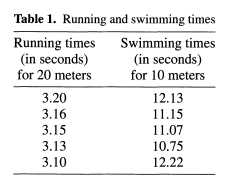
\includegraphics[width=50mm]{experimentTable.png}
  \label{fig:path1}
  \end{center}
\end{figure}\\
After the trials above, we choose the three optimal running and swimming times for Elvis and get their average $$r=6.4m/s \quad and \quad s=0.910m/s$$.\\
Then we have $$(2) \Rightarrow y = 0.144x \quad (3)$$\\ \newpage
Following the above preparation, is the experiment. Below there is the table of Elvis' throw and fetch trials and the scatterplot of the tables data.  
\begin{figure}[h!]
  \begin{center}
  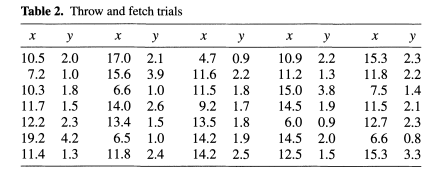
\includegraphics[width=100mm]{throwFetchTrials.png}
  \label{fig:path2}
  \end{center}
\end{figure}\\


  \begin{center}
\begin{figure}[h!]
  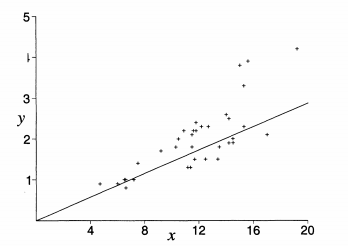
\includegraphics[width=100mm]{ElvisChoice.png}
  \caption{Scatter Plot of Elvis's choices with optimal line}
  \label{fig:path3}
	\end{figure}
  \end{center}

In figure 2 we clearly see that most of the points show a rather tight and clear pattern, or as statisticians would call it, smooth. \\In the same figure we also see the line we predicted from the model we created, $y = 0.144x.$ \newpage
\begin{center}
\textbf{Assumptions}\\
\end{center}
\textbf{1.}There was a definite line between shore and lake. Because of waves, this
was not the case\\
\textbf{2.}When Elvis entered the water, he started swimming. Actually, he
ran a short distance in the water.\\
\textbf{3.}The ball was stationary in the water\\
\textbf{4.}The values of r and s are constant, independent of the distance run
or swum.\\ \\
\textbf{Note:} There is the possibility that Elvis chose paths actually \textit{better} than the optimal we predicted\\
\begin{center}
\textbf{Conclusion}\\
\end{center}
\textbf{1.} We use a mathematical model.\\
\textbf{2.} To arrive at the theoritical figure we made all of the above simplifying assumptions\\
\textbf{3.} There is always the possibility of an error in measurements\\

However, despite all of the above, Elvis does not know calculus. In fact, he has trouble differentiating even simple polynomials. More seriously,
although he does not do the calculations, Elvis's behavior is an example of the uncanny way in which nature (or Nature) often finds optimal solutions. Consider how
soap bubbles minimize surface area, for example. It is fascinating that this optimizing
ability seems to extend even to animal behavior. (It could be a consequence of natural selection, which gives a slight but consequential advantage to those animals that
exhibit better judgment.) 
}

\end{document}  	